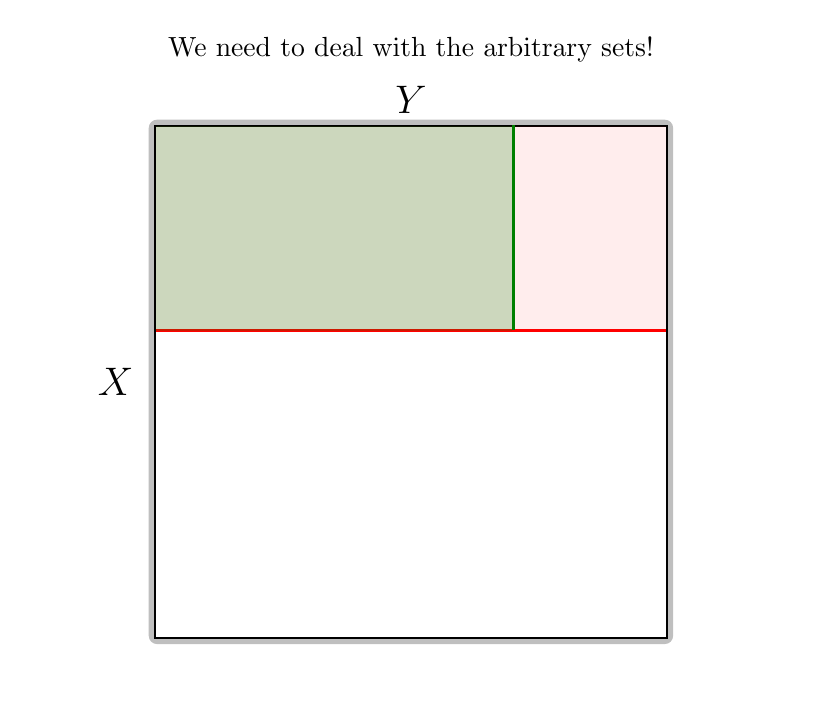
\begin{tikzpicture}
    \def\n{9}
    \def\m{9}
    \def\step{0.65}

    \node at (-1.5, 0) {};
    \node at ({\step * (\m + 1) + 1.5}, 0) {};


    \fill[gray!50, rounded corners = 3pt] (-0.08, 0.08) rectangle
        ({\step * (\n + 1) + 0.08}, {-\step * (\m + 1) - 0.08});
    \fill[white] (0, 0) rectangle ({\step * (\n + 1)}, {-\step * (\m + 1)}); 
    \draw[thick] (0, 0) rectangle ({\step * (\n + 1)}, {-\step * (\m + 1)});
    \node at ({\step * 4}, {-\step * (\m + 1) - 0.56}) {};

    \uncover<2->{
        \draw[very thick, red] (0.01, -4 * \step) --
            ({\step * (\n + 1) - 0.01}, -4 * \step);
    }

    \uncover<3->{
        \fill[red, opacity = 0.07] (0.01, 0) rectangle
            ({\step * (\n + 1) - 0.01}, -4 * \step);
    }

    \uncover<4->{
        \draw[very thick, green!50!black] (7 * \step, 0.01) -- (7 * \step, {-\step * 4 + 0.01});
    }

    \uncover<5->{
        \fill[green!50!black, opacity = 0.2] (0.01, 0) rectangle
            ({\step * 7 - 0.01}, -4 * \step);
    }

    \uncover<6->{
        \node at ({\step * (\m + 1) / 2}, 3 * \step / 2) {\alert{We
                need to deal with the arbitrary sets!}};
    }

 
    \node at (-0.5, {-\step * (\m + 1) / 2}) {\Large $X$};
    \node at ({\step * (\m + 1) / 2}, \step / 2) {\Large $Y$};

\end{tikzpicture}